\documentclass[a4paper,10pt]{article}
\usepackage[utf8]{inputenc}
\usepackage{graphicx}

\title{Poetry Generator Report}
\author{Kyle Maclean}
\date{July 2021}

\begin{document}

\maketitle

\texttt{https://github.com/KyleMaclean/Poetry-Generator.git}
\newline

\section{Core Ideas}

\begin{figure}[htb!]
\centering
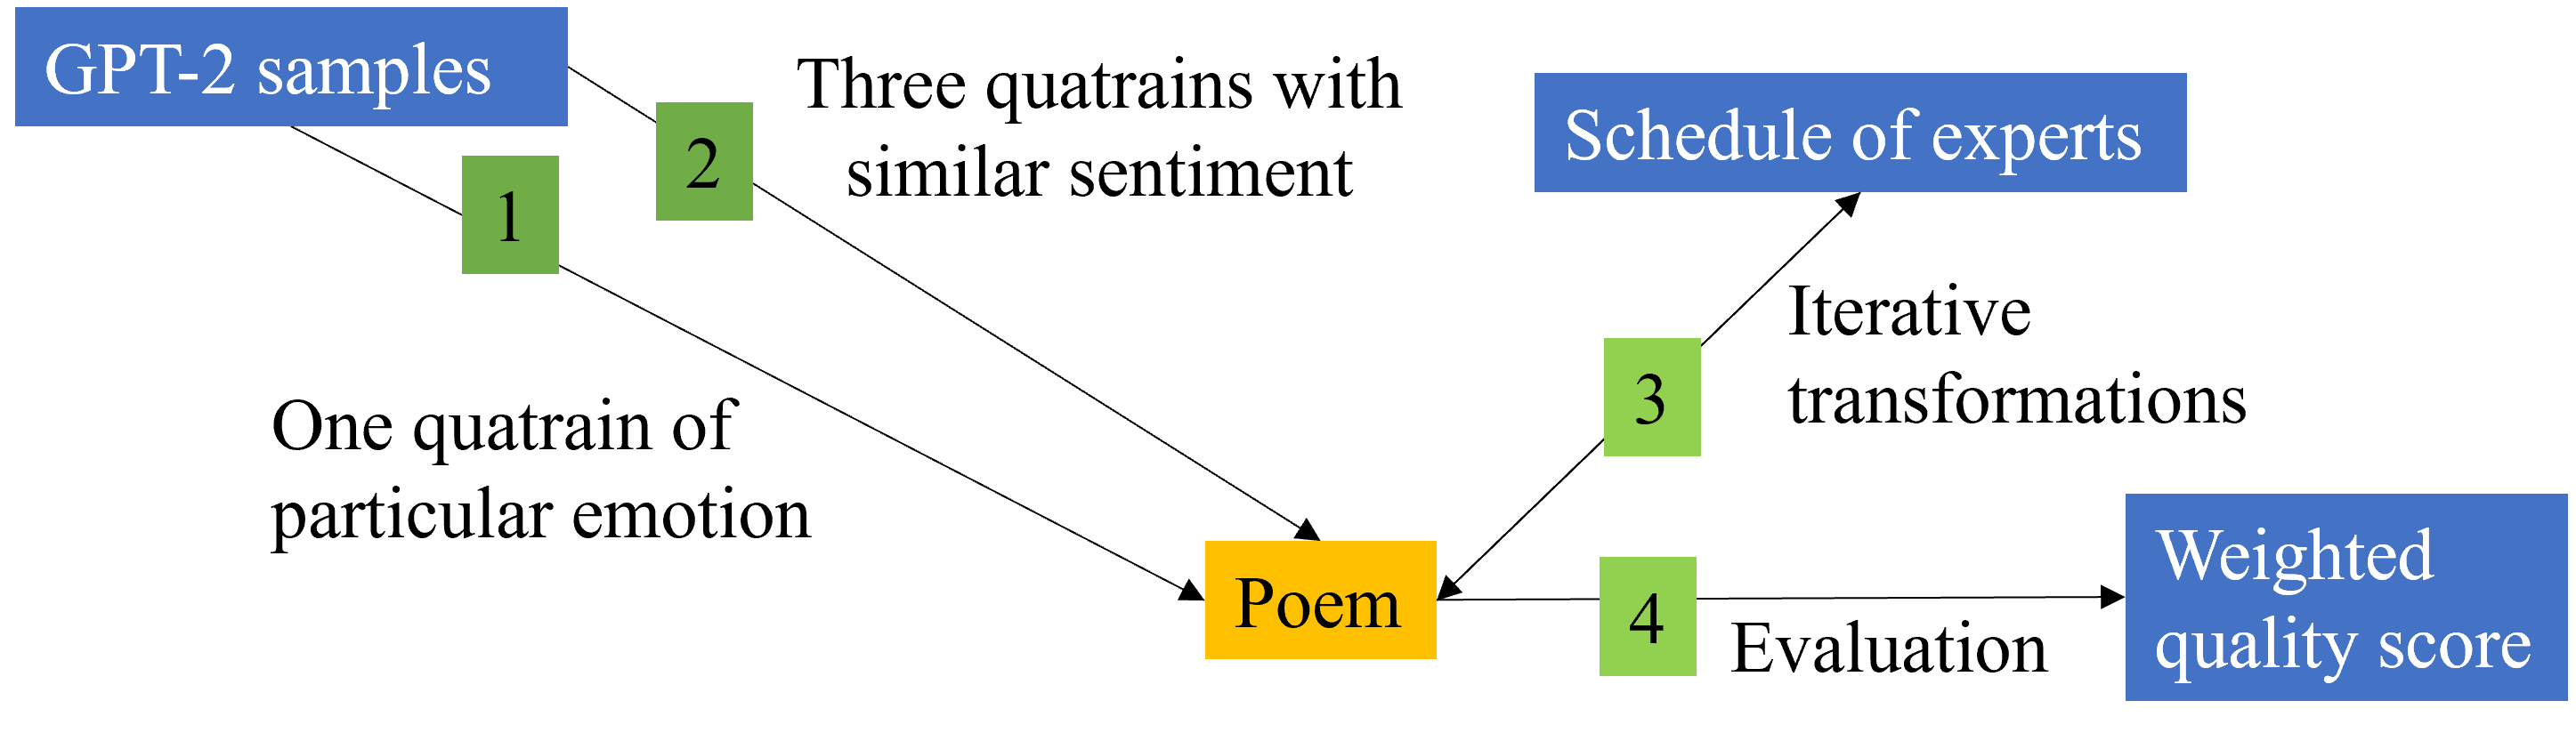
\includegraphics[width=1\textwidth]{media/core-ideas-diagram.png}
\caption{High-level illustration of the system.}
\label{fig:core-ideas-diagram}
\end{figure}

We present a system which generates high-quality poems. Figure \ref{fig:core-ideas-diagram} shows how it receives a single quatrain as an input "prompt" and then chooses three more quatrains which suit it from a machine-generated corpus of poetry samples. For testing purposes, different prompts were selected to represent a diverse range of emotions. A copy of the Generative Pre-trained Transformer 2 (GPT-2) \cite{budzianowski_hello_2019} was retrained on English poems to generate this corpus. The four quatrains are then transformed by iteratively applying a list ("schedule") of natural-language processing programs ("agents"). The final poem quality \cite{jordanous_evaluating_2013} is determined by a weighted sum of:
\begin{itemize}
    \item RHYME:
    \begin{itemize}
        \item FREQUENCY: ratio of couplets which rhyme compared to those that do not.
        \item LEVEL: how many ending phonemes match at the ends of two lines which are part of a couplet.
    \end{itemize}
    \item ALLITERATION
    \begin{itemize}
        \item CHAIN: length of the longest chain of consecutive alliterative words.
        \item TOTAL: total number of alliterations.
    \end{itemize}
    \item PHONEME: phoneme length consistency in each couplet.
\end{itemize}

\section{Question to be Answered}

The motivating question which shall be addressed by answering related sub-questions in § \ref{discussion} is: "How is poem quality affected by different agents and different schedules of applying such agents?"

\section{Literature Review}
% •	background research and how you have used it to contextualise your work

Previous poem generation work includes using distinct components to define grammar, understand semantics, etc., to place constraints on a search space of possible words and lines \cite{toivanen2012corpus} \cite{toivanen2013harnessing} and an agent-based approach which did not have a shared medium between the agents and requires them to interact to influence each others' state, which is the only "memory" \cite{astigarraga_emotional_2017}.

Our work is primarily inspired by a shared workspace ("blackboard") system \cite{misztal-radecka_blackboard_2016} \cite{hayesrothblackboard1985} where agents operate on text according to some schedule to yield a poem. It is based upon the the Global Workspace Theory of Mind \cite{baars_theater_2001} \cite{Baars2003BAATGB} which states that tasks in our minds can be considered to be undertaken by many autonomous agents. Simulating this in software could use a central datastructure of text which is maintained by the system while different subsystems (agents) operate upon it. It is appropriate that this architecture was originally developed for speech understanding \cite{ERMAN1981349} \cite{carver_evolution_1994} because our problem domain also has to do with natural language.

Character-level recurrent neural networks ("char-RNNs") have been used in various text/music generation scenarios \cite{malik_music_2021}. In particular, a system for generating Chinese classical poetry was able to demonstrably learn structural elements, rhythm and semantics \cite{yi_generating_2017}. Char-RNNs predicts the next character in some text, learning from whether it can successfully reproduce some given training text. However, Transformer Networks, which are based solely on attention mechanisms, have been shown to produce more interesting text than Char-RNNs \cite{branwen_rnn_2015}. The intuition is that "attention is all you need" and that recurrences need not be used at all \cite{vaswani_attention_2017}. Accordingly, we chose the Transformer Network, GPT-2.

The GPT networks often achieve the best performance in language modelling benchmarks \cite{language_modelling_benchmarks}. GPT-2 in particular was shown in 2019 to have state-of-the-art results on 7 out of 8 datasets in a zero-shot setting. Such a flexible and high-performing network would be beneficial for our project because we require transference to the somewhat niche domain of poetry generation. Since GPT-2 is so powerful, OpenAI has a complicated policy of releasing smaller versions of it to the public to curtail the generation of fake news, hate speech, etc. \cite{solaiman_release_2019}. We found experiments conducted on three versions with different numbers of parameters: 117 million, 345 million, and 1.5 billion, with the bigger models producing better results when trained properly \cite{branwen_gpt-2_2019}. These experiments trained on a combined dataset of Project Gutenberg poems and a collection of contemporary poetry from the Poetry Foundation \cite{foundation_poems_2021}.

\section{Environment and Agent Design}
% •	the choice of task environment and how you have used it/adapted it for your specific project

The sample space of GPT-2 poems is divided into quatrains. Using a map from a large number of emotional words to a small number of emotions describing each word, the former is found in the set of quatrains to tag that quatrain as a prompt with the latter. 25 prompts representing distinct emotions were found in our corpus.

To find the other three quatrains for the rest of the poem, the sentiment of each prompt is analysed to search through 10\% of the randomly-shuffled corpus and return a quatrain with the closest sentiment (in Euclidean distance) to the prompt. The sentiment of the two is used to find the third, and of the three to find the fourth. Although the quatrains are "found", it is also suitable to say that they are "generated" since the itself is machine-generated; it can be thought of as a constrained/filtered generation procedure.

To compare the schedules, the randomness in generating the quatrains is fixed, so that each schedule starts with identical poems.

\section{Implementation}
\label{sec:implementation}
% •	the effective use of artificial intelligence and agent-based systems ideas from the course and your wider studies in designing your autonomous agents
% technologies used and implementation challenges

The Python implementation treats each schedule as an ordered list, where each element is a pair of the agent function (from \texttt{agents/}) and a helper function according to whether the agent operates on a single line, a couplet, or all the lines of the poem. The dictionary of all schedules is in \texttt{allocator.py}, where each is named after a Greek letter.

Each agent uses a combination of its own code and utilities which are shared between multiple agents in \texttt{util/}, all of which largely builds upon the NLTK library \cite{xue_2011}. Perhaps the most efficient way to understand the workings of the agents is be to examine their unit tests, so § \ref{ssec:samples-of-agent-outputs} contains one for each agent. Also, reading their source code is straightforward because of the high levels of abstraction afforded by the extracted utility functions.

To generate prompts, \texttt{emotion\_cardinality\_reducer.txt} \cite{emotion-cardinality-reducer-github} is used as a map from a word found in \texttt{gpt2\_samples.txt} to an emotion to select that words contextual quatrain as an instance of one of the emotions.

NLTK's built-in corpora have large search spaces, making computation time prohibitive for the agents to use them. For example, \texttt{nltk.corpus.cmudict} has 133,737 entries and \texttt{nltk.corpus.brown} \cite{francis1979brown} has 11,611,192 words. Using the top 1000 most common English words resulted in boring output because of the lack of diversity. We needed something in between and thus created a custom corpus, stored in \texttt{words\_pos\_phonemes\_9802.py}. It was derived by starting with The Online Plain Text English Dictionary \cite{OPTED} of 54,555 words and finding the intersection of non-duplicated words with the CMU Pronouncing Dictionary \cite{CMUpd} to tag them with their constituent phonemes. \texttt{nltk.pos\_tag} was used to tag them with their parts of speech.

\section{Experiment Design}
% •	how clear your question(s) are, how well the experiments have been designed to answer them, and your level of rigour in planning and analysing the experiments

We pre-generated the GPT-2 samples because there is no benefit in doing so on-the-fly and only slows the process down significantly. Out of all the versions of GPT-2 that OpenAI released, we chose the biggest, GPT-2-1.5B, which has 1.5 billion parameters \cite{solaiman_release_2019}. By intuition, a model with more parameters is capable of generating more complex poetry (this has also been shown experimentally too \cite{branwen_gpt-2_2019}). It is preferable for us because we are generating a lot of poems and we do not want them to become repetitive. Performing inference on such a model at run-time is infeasible, especially because we do a lot of experiments to examine the effects of different hyper-parameters.

We pre-generated a dictionary of prompts for each emotion using \texttt{get\_n\_prompts.py} and used the same prompts for each set of experiments, except when determining the effect on quality of different random seeds, and therefore different prompts (§ \ref{ssec:random-seed-comparison}).

Each schedule is evaluated by the quality of the poems it creates given 25 prompts conveying distinct emotions. The weighting of the quality evaluation procedure is calibrated to give greater importance to some components. This can only reflect a human's subjectivity as to what a high-quality poem is, so the author manually tuned them to give what he perceived to be better poems higher scores. The weights are: 'RHYME' (including 'FREQUENCY' and 'LEVEL'): 100, 'ALLITERATION CHAIN': 50, 'ALLITERATION TOTAL': 5, 'PHONEME': 1. The weights partially address the fact that the evaluation function outputs are not zero-normalised because it is difficult to do so objectively, therefore it is also difficult to engineer the weights to represent a precedence of the different quality descriptors.

Quality is greatly affected by initial randomness so it is futile to attempt to tune agent hyper-parameters to maximise quality. Specifically, if the initial quatrains happen to have many couplets which are easily rhymed through synonym replacement, then schedules of agents which exploit this will perform well. Conversely, if there are few opportunities to rhyme but lots of adjectives before nouns, it may be easier for the alliteration agents to replace such words with alliterative ones. Therefore, the experiments consist of answering performance-related questions with data.

\section{Results and Discussion}
\label{discussion}
% •	how well the report answers the question by using the evidence from the experiments
% discussion of question in light of results

\subsection{Do agents which were designed to increase poem quality actually increase poem quality while preserving semantics?}
\label{label:baseline-quality-increase}

\begin{figure}[htb!]
\centering
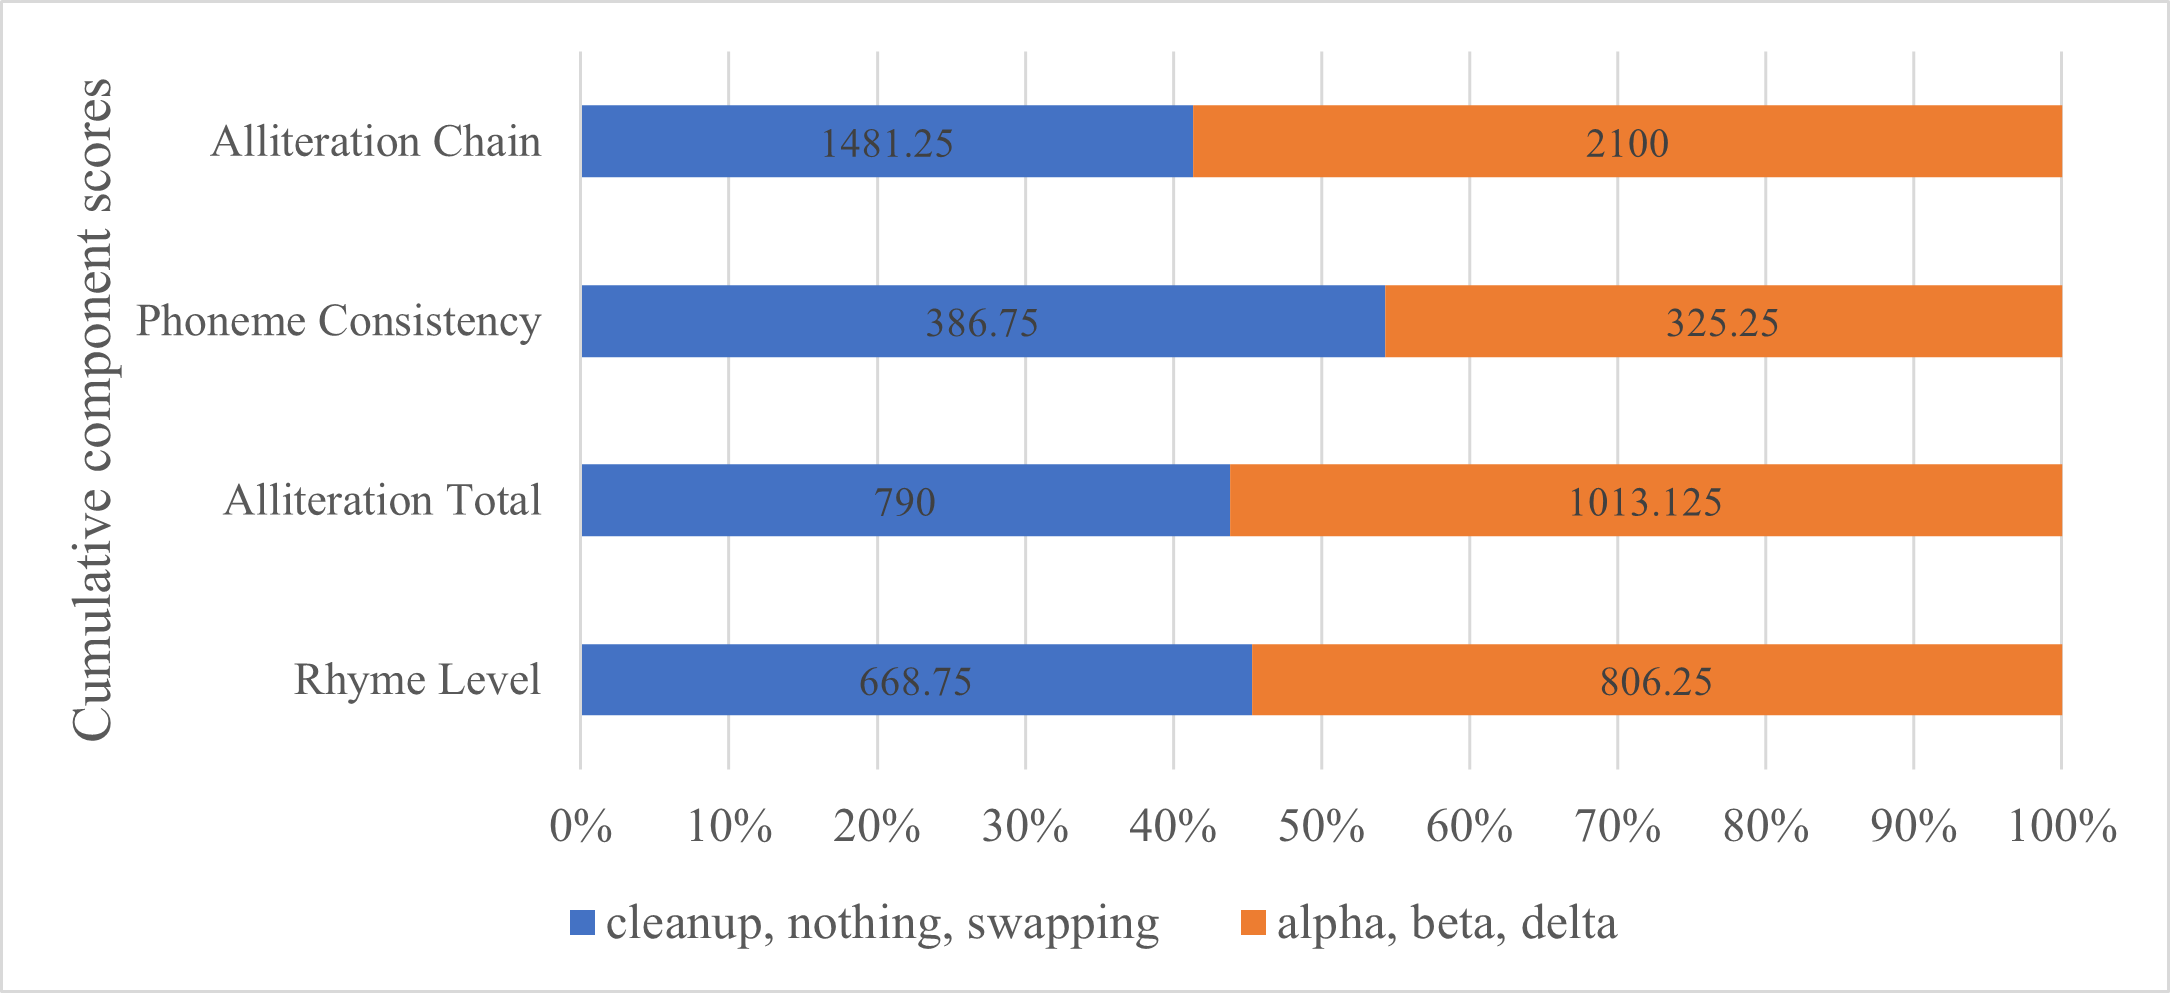
\includegraphics[width=1\textwidth]{media/baseline-quality-increase.png}
\caption{The relative component scores of poems after using agents which we expect to not increase quality versus agents which we do expect to increase quality. Each coloured bar is a cumulative sum of the specified component scores for 75 poems: 25 for each emotion and 3 schedules: [cleanup, nothing, swapping] (the dummy schedules which are not expected to increase quality) and [alpha, beta, delta] (the schedules which are expected to increase quality). See \texttt{data/baseline-quality-increase.xlsx} for the source data.}
\label{fig:baseline-quality-increase}
\end{figure}

We verify that the best three of the first five schedules produce poems of higher quality than dummy schedules which either just correct an/an/punctuation ("cleanup"), or do nothing ("nothing"), or swap conjugates/couplets ("swapping"). They all preserve semantics because word replacements can only be synonyms.

Ranking the first five schedules according to cumulative poem quality for 25 emotions: delta: 1541.375, alpha: 1532.125, beta: 1171.125, epsilon: 1157.75, gamma: 1155.375. See \texttt{data/baseline-quality-increase.xlsx} for the source data.

In Figure \ref{fig:baseline-quality-increase}, we see that the three best schedules produce significantly higher scores than the dummy schedules except in phoneme consistency. Therefore, agents are capable of increasing alliteration and rhyme frequency. Phoneme length may have become inconsistent because the agents may lengthen some lines more than others in trying to maximise the other quality components. Also, none of the best schedules contained an agent which maximises phoneme consistency, such as the \texttt{equalise\_line\_length} agent. Before transformation, the poems already had decent phoneme length consistency because they were generated by a copy of GPT-2 which was retrained on poems written by humans, most of which consist of couplets of lines of similar lengths.

\subsection{Does increasing the number of schedule iterations increase poem quality?}
\label{sec:iteration-quality-box-whisker}

\begin{figure}[htb!]
\centering
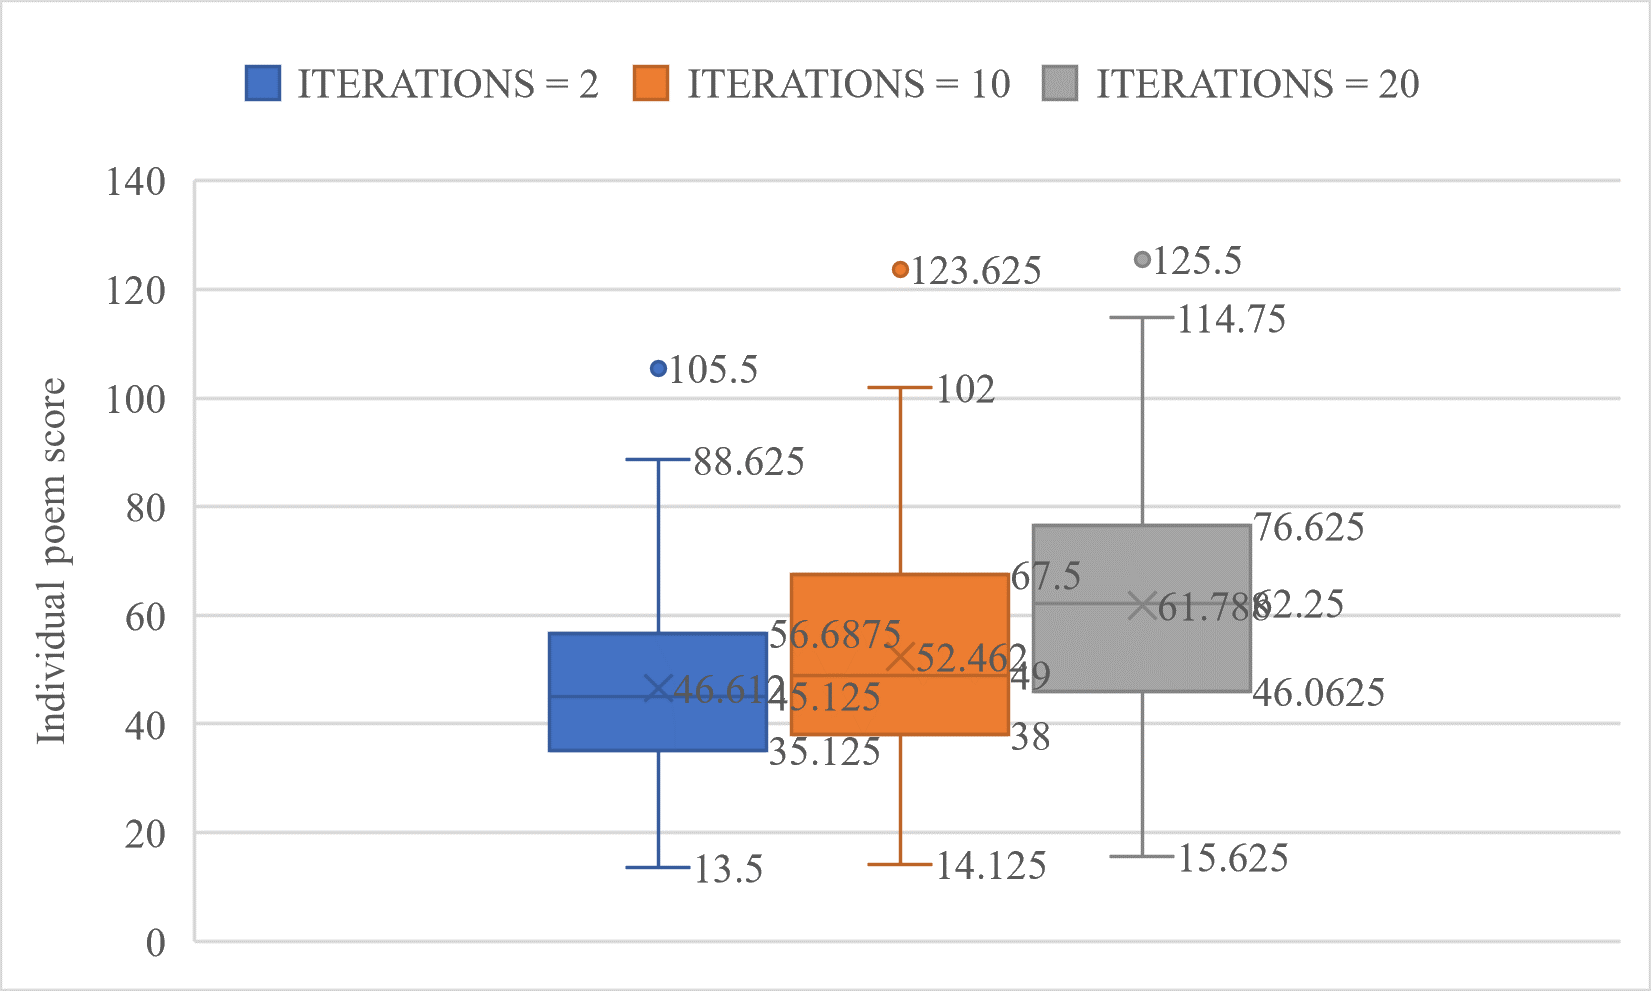
\includegraphics[width=1\textwidth]{media/iteration-quality-box-whisker.png}
\caption{Box and Whisker Plot showing statistical differences between poem quality according to how many times the schedules of agents were applied. Each box is an aggregate of the scores of 125 poems: 25 for each emotion and 5 schedules (alpha to epsilon). See \texttt{data/iteration-quality-box-whisker.xlsx} for the source data.}
\label{fig:iteration-quality-box-whisker}
\end{figure}

Figure \ref{fig:iteration-quality-box-whisker} shows that poem quality increases with more iterations. A two-tailed, paired T-Test can be used to verify this because the difference may be in either direction and corresponding poems in each set of experiments were generated by the same initial random process. Between the 2- and 10-iteration experiments, the p-value is 6.001E-5 and between the 10- and 20-iteration experiments, the p-value is 1.409E-10. Assuming $\alpha$ = 0.05, both p-values are less than $\alpha$, and therefore we may reject the null hypothesis, implying that there is a statistically significant difference in quality when increasing iterations from 2 to 10 and 10 to 20, in support of the hypothesis.

\subsection{How do the component scores of the extraordinarily high quality poems compare to the others?}

\begin{table}[htb!]
    \centering
    \begin{tabular}{|l|l|l|l|}
    \hline
        & "105" ranking & "123" ranking & "125" ranking \\ \hline
        Rhyme Level & 1 & 1 & 1 \\ \hline
        Alliteration Chain & 36 & 4 & 1 \\ \hline
        Alliteration Total & 25 & 14 & 44 \\ \hline
        Phoneme Consistency & 70 & 16 & 98 \\ \hline
    \end{tabular}
    \caption{The ranking for each component score (out of 125) for the three poems whose overall quality scores were high outliers. See \texttt{data/delta-outlier-examination.xlsx} for the source data.}
    \label{tab:delta-outlier-examination}
\end{table}

To better understand the influence of our score weights, we examine the weighted component scores of the three outlier poems shown in Figure \ref{fig:iteration-quality-box-whisker} as dots. They shall be referred to as, "105", "123", and "125", after their scores. All of them were generated by the delta schedule, and we also note that the delta schedule produced the highest quality poems in aggregate in the 10-iteration experiments, as shown in § \ref{label:baseline-quality-increase}. We note from Table \ref{tab:delta-outlier-examination} that all three outliers had the best rhyme level scores and that their worst-ranked scores were phoneme consistency. This suits the subjective preferences of the author, who thinks that rhyming is the most important aspect of poem quality and phoneme consistency is the least important, with alliteration being somewhere in between.

\subsection{Were the results consistent when generating the initial quatrains with a different random seed?}
\label{ssec:random-seed-comparison}

We ran a set of 10-iteration experiments, using the same emotional prompts but with a different random seed initialised in the Allocator. This caused the GPT-2 samples to be shuffled differently and therefore caused different quatrains which satisfy the sentiment similarity requirement to be chosen. Agents which use randomness were also affected because their seed is given as a parameter by the Allocator. For each seed, we ran each of the first 5 schedules (alpha - epsilon) on the 25 emotion prompts, generating 125 poems. For seed=42, the sum of scores is 6557.75 and for seed=43, the sum of scores is 6624.625. These seem quite similar. To verify this a two-tailed, paired T-Test is used for the same reasons described in § \ref{sec:iteration-quality-box-whisker}. The resulting p-value is 0.822539055. Assuming $\alpha$ = 0.05, this value is greater than $\alpha$ and therefore we fail to reject the null hypothesis, implying that the difference in performance using different seeds is likely due to random chance. The choice of random seed does not affect poem quality significantly. See \texttt{data/random-seed-comparison.xlsx} for the source data.

\subsection{Can quality be increased by not maintaining semantics?}

\begin{figure}[htb!]
\centering
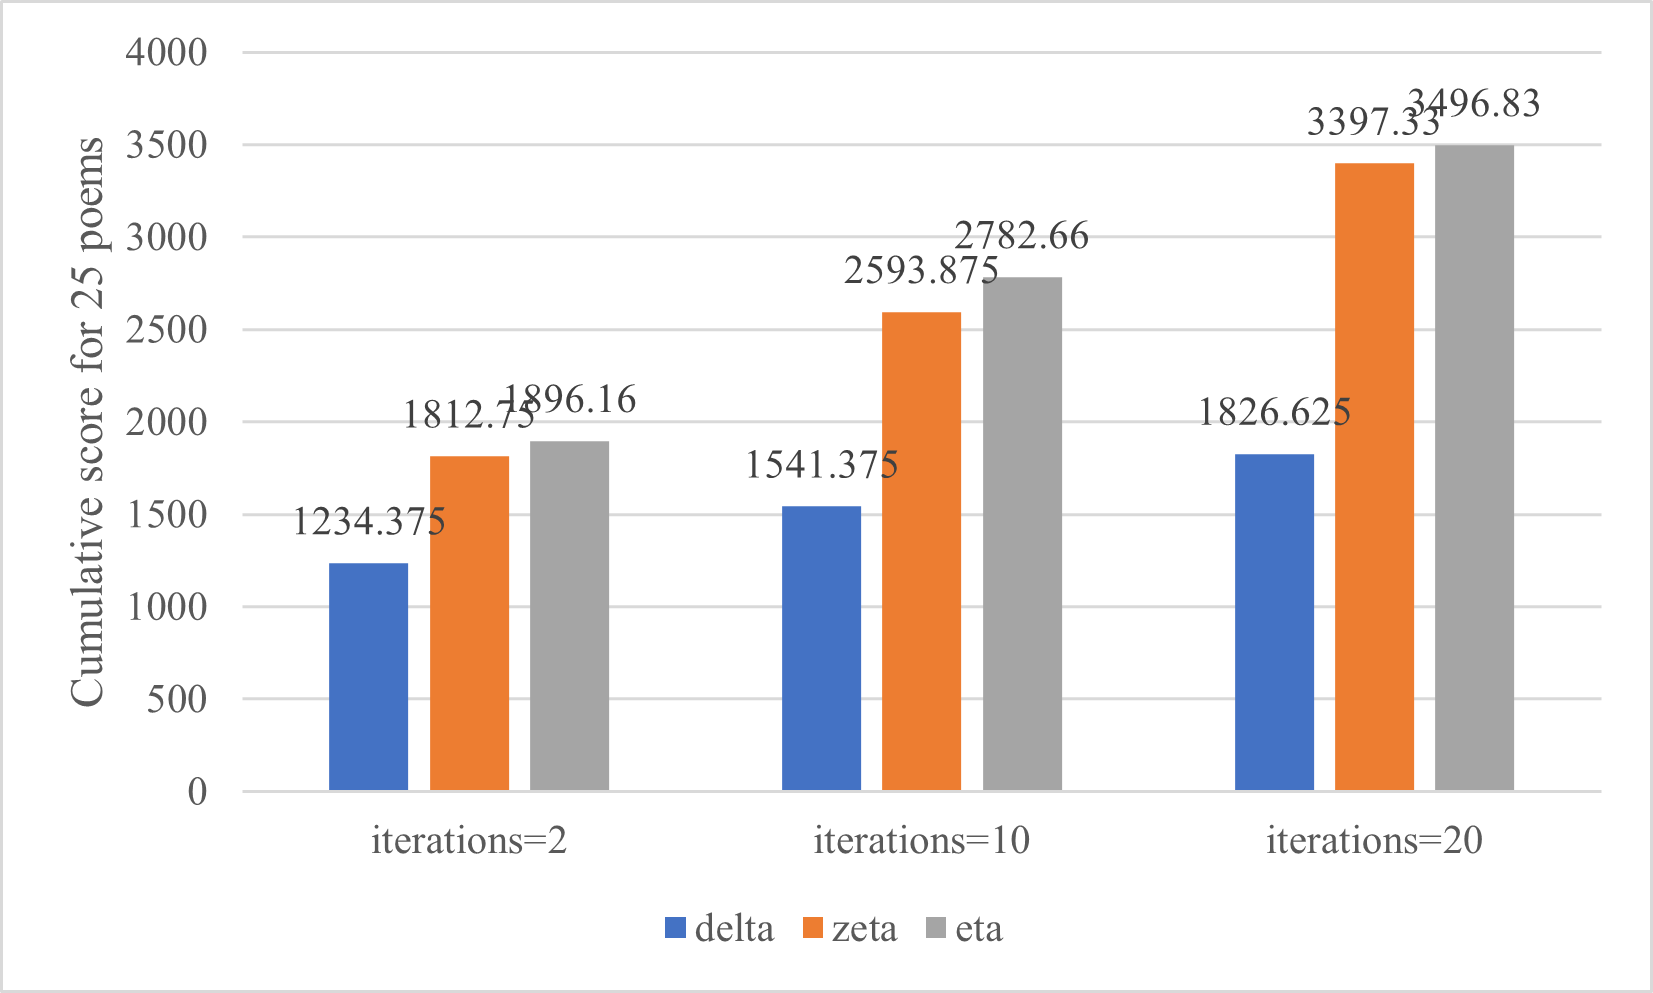
\includegraphics[width=1\textwidth]{media/arbitrary-evaluation-overall.png}
\caption{Comparing the best of the first 5 semantics-preserving schedules (delta) with the two schedules that use the arbitrary rhyme and alliteration agents. See \texttt{data/arbitrary-evaluation-overall.xlsx} for the source data.}
\label{fig:arbitrary-evaluation}
\end{figure}

Schedule zeta is a copy of delta except with the agents \texttt{alliterate\_line\_synonymously} and \texttt{rhyme\_two\_lines\_synonymously} replaced with \texttt{alliterate\_line\_arbitrarily} and \texttt{rhyme\_two\_lines\_arbitrarily} respectively. Schedule eta only has the latter agents. The results in Figure \ref{fig:arbitrary-evaluation} are as expected because the agents' alliteration and rhyme search spaces are much less constrained when not having to use synonyms. To demonstrate how prolific the alliteration is, here are some selected lines from the poems generated by these agents:

\begin{verbatim}
    - gravelly gullible got she and goodly gorgeous grew she
    - for saliva, his sacrilegious sake
    - Speak out, and let legacies leave lifted.
    - faintly fundamental they fell
    - Dew'd the salesmen until their sabbatical scotch,
    - To feed a neurotic and nestorian nickle's note
    - And groceries of greater ghastliness than our gothic grid?
    - Of their neurotic ninetieth, we knelt and grieved
    - find out fluently, and would federalize his foursquare
    - A ritualistic red-handed recluse
\end{verbatim}


\subsection{Can an agent significantly increase couplet phoneme consistency?}

\begin{figure}[htb!]
\centering
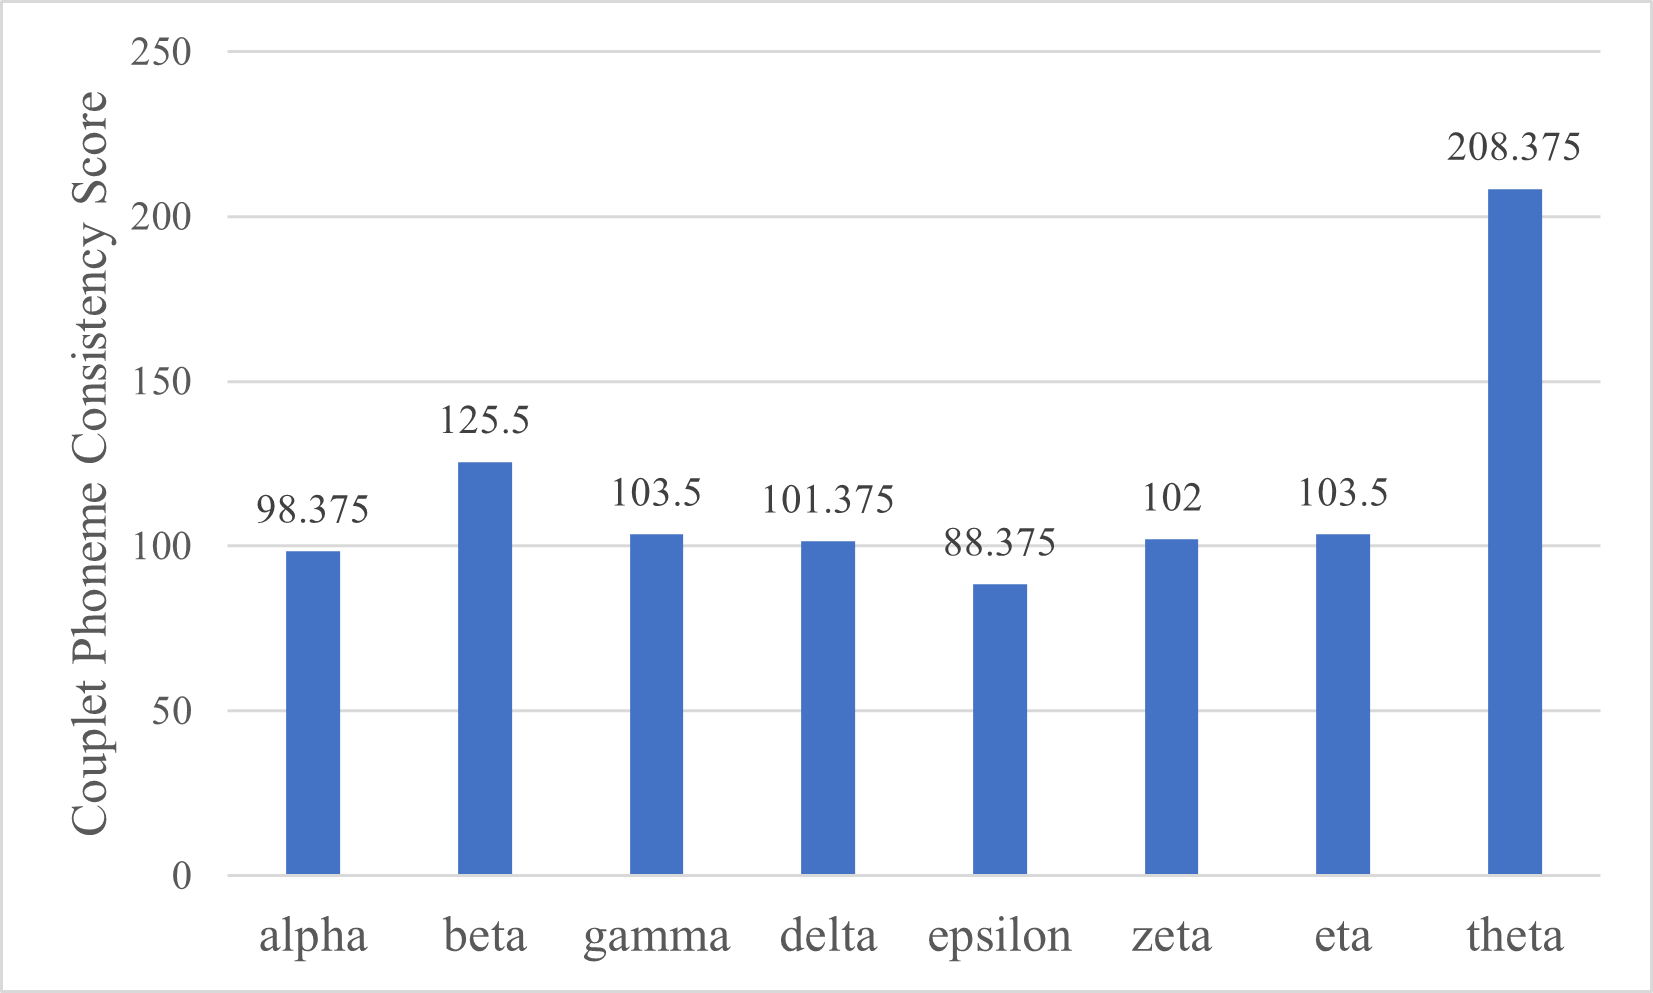
\includegraphics[width=1\textwidth]{media/theta-component-phoneme.png}
\caption{The cumulative Couplet Phoneme Consistency Scores for poems generated from 25 different emotion prompts by each of the schedules which do not use the \texttt{equalise\_line\_length} agent (alpha - eta) and the schedule which only consists of that agent (theta). See \texttt{data/theta-component-phoneme.xlsx} for the source data.}
\label{fig:theta-component-phoneme}
\end{figure}

Schedule theta only applies the agent \texttt{equalise\_line\_length}, which is designed to maximise phoneme consistency in random couplets of the poem. From the results of Figure \ref{fig:theta-component-phoneme}, we see that it achieves approximately twice the phoneme consistency of all the other schedules. Therefore, agents can significantly increase couplet phoneme consistency. \texttt{equalise\_line\_length} is often unable to achieve consistency within EPSILON=3 phonemes before "Attempt 4" (see the source code). In these cases, as its last resort, it simply chops words off the end of the longer line. When this happens, the poem loses semantics and grammatical coherency. However, if we remove that last resort step, then the agent fails to get the number of phonemes within EPISLON=3 for many couplets. Therefore, \texttt{equalise\_line\_length} seems unable to significantly increase phoneme consistency without these trade-offs.

\section{Conclusion}
% conclusion; summary; successes and limitations; brief address of future work
% •	the quality of reflection on the successes and limitations of the work

Our system can be configured to produce poems with specific emotions, alliteration schemes, rhyme frequency and phoneme consistency. They are often grammatically coherent and sometimes funny. The question was answered using data-driven analysis. Trade-offs can be made between semantics maintenance and quality maximisation. The prompts from GPT-2 tend to drift between themes arbitrarily, so to use this system for augmenting/extending a human poet's work in which semantics should be maintained, it might be worth using the "synonymous" instead of "arbitrary" agents.

There are many paths for future work:
\begin{itemize}
\item More schedules could be developed which incorporate the unused agents. Only 15 agents were used out of the 19 that were developed.
\item Schedules could be developed which do not simply iterate over an ordered list but use sub-schedules which are applied according to the state of the poem or the progress within the budget of computations.
\item Runtime could be measured to inform uses where it is relevant by considering the effects of, for example, corpus size.
\item Another layer of abstraction could be placed in between agents and schedules to implement the wildcards in \cite{VealeCreativeLanguageRetrieval}.
\item Agents which accomplish different NLP tasks could be developed.
\item Different quality components could be measured and different weight could be assigned to emphasise poems which are better by other metrics and focus development on agents which optimise for them.
\item Prompts could be given by humans and quatrains could be selected from human-created and human-curated emotion/theme categories.
\item More intelligent grammar and semantics analysis and manipulation can be used to improve the \texttt{equalise\_line\_length} agent to decrease the rate at which it needs to chop lines short.
\end{itemize}


\section{Appendix}

\subsection{Video demonstration}

\begin{figure}[htb!]
\centering
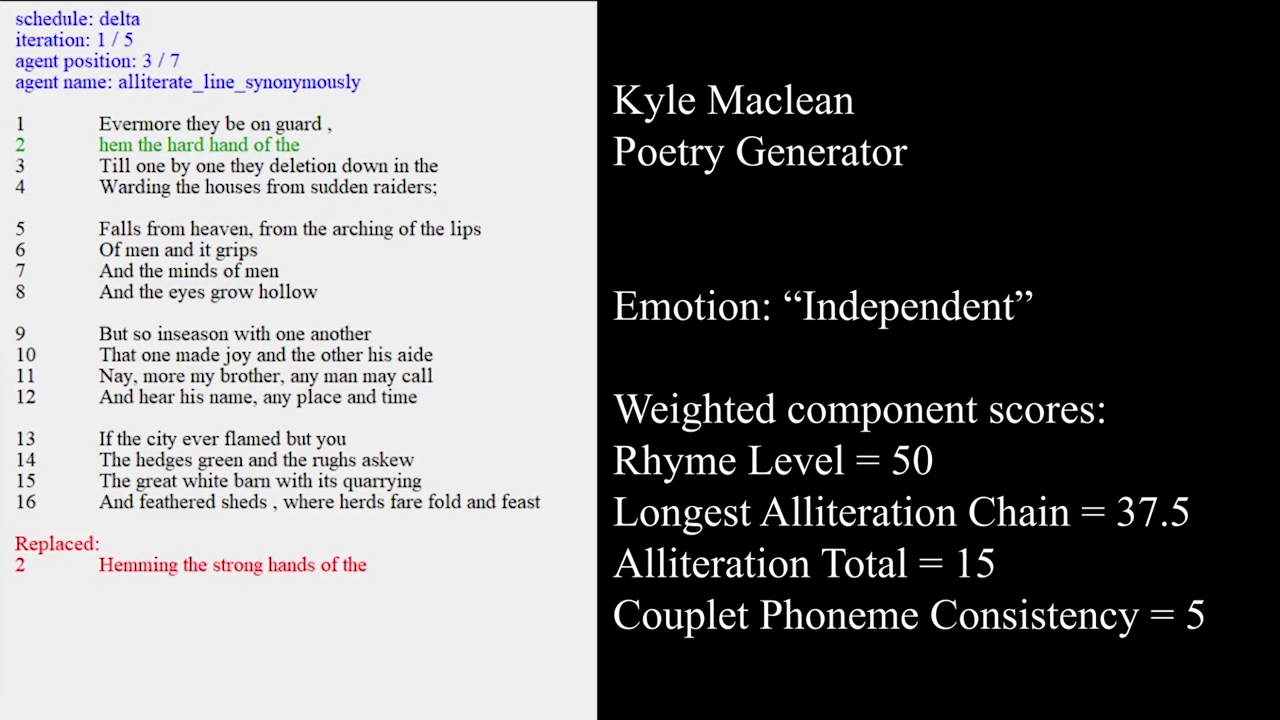
\includegraphics[width=1\textwidth]{media/demo-snapshot.png}
\caption{Snapshot from the video demonstration which shows the result of applying the agent \texttt{alliterate\_line\_synonymously} to replace "strong hands" with "hard hand".}
\label{fig:demo-snapshot}
\end{figure}

\texttt{demo\_psykjm\_14327105.mp4} is a demonstration of the system generating and transforming a poem, a snapshot of which is shown in Figure \ref{fig:demo-snapshot}.

\subsection{Samples of agent outputs}
\label{ssec:samples-of-agent-outputs}
Below is an interaction with the system using some of the 60 tests cases from \texttt{tests/} to demonstrate the agents operationally.
\begin{verbatim}
>>> from agents import *

>>> a_an_correction(['it is an mistake', 'to see a elephant'])
['it is a mistake', 'to see an elephant']

>>> add_metaphor('you are beautiful')
'you are beautiful as the vivid colors of a painting'

>>> add_sensible_adjectives('the bread and wine')
'the white bread and wine'

>>> alliterate_line_synonymously('hello world')
'hi humanity'

>>> couple_existing_rhymes(['there was a cat', 'and a roof', 'on which it sat'])
['there was a cat', 'on which it sat', 'and a roof']

>>> decrease_to_single_adjective('it was a hot, sunny, windy day')
'it was a sunny day'

>>> equalise_line_length(['eating from a big bowl of strawberries', 'on the blanket'])
['eating from a bowl of strawberries', 'on the visible radiation blanket']

>>> punctuation_spacing_correction(['there was a mouse , cat , dog and flower !'])
['there was a mouse, cat, dog and flower!']

>>> remove_random_adjective('i saw a bright light')
'i saw a light'

>>> remove_unrhymable_couplet(['a patch of silver', 'on the orange'])
[]

>>> replace_with_antonym('we saw the happy Heffalump')
'we saw the unhappy Heffalump'

>>> replace_with_hyponym('the apple is on the floor')
'the crab apple is on the floor'

>>> replace_with_synonym('we discovered a new realm')
'we discovered a new kingdom'

>>> replace_with_synonym_of_synonym('today is a huge day')
'today is a vast day'

>>> rhyme_two_lines_arbitrarily(['trees like you', 'are very tall'])
['trees like you', 'are very new']

>>> rhyme_two_lines_synonymously(['there was a mouse', 'in his home'])
['there was a mouse', 'in his house']

>>> swap_conjugates(['red apple and yellow pear'])
['yellow pear and red apple']

>>> swap_couplets(['all on its own', 'we found a house', 'in the forest', 'with a box'])
['in the forest', 'with a box', 'all on its own', 'we found a house']

\end{verbatim}


\bibliographystyle{unsrt}%Used BibTeX style is unsrt
\bibliography{bib}

\end{document}
